\documentclass[a4paper,12pt]{article}
\usepackage[utf8]{inputenc}
\usepackage[T1]{fontenc}
\usepackage[a4paper, margin=1in, bindingoffset=6mm]{geometry}
\usepackage{lmodern}
\usepackage{upgreek}
\usepackage{bm}
\usepackage{graphicx}
\providecommand{\e}[1]{\ensuremath{\times 10^{#1}}}
\usepackage{siunitx}
\usepackage[export]{adjustbox}
\graphicspath{ {Images/} }
\usepackage{placeins}
\usepackage{epstopdf}
\usepackage{subfigure}
\usepackage{pstricks}
\usepackage{epsfig} % extra package for .eps graphics usage
\usepackage{pst-grad} % For gradients
\usepackage{pst-plot} % For axes
\usepackage{amsmath} % extra math symbols There are a lot of amps packages
\usepackage{fancyhdr} % to use fancy headers and footers --- requires for most professional docs
\usepackage{watermark} % to include a figure in the background - the front page for example
\usepackage{enumerate} % to enumerate your items in a list with any style
\usepackage{booktabs}
\usepackage{siunitx}
\usepackage{wallpaper}
\usepackage{afterpage}
\usepackage{mathrsfs}
\usepackage{gensymb}
\usepackage{textcomp}
\usepackage{color}
\definecolor{mygreen}{RGB}{28,172,0}
\definecolor{mylilas}{RGB}{170,55,241}
\usepackage{listings}
\usepackage{pdfpages}

\usepackage[framed,numbered]{matlab-prettifier}

% \lstset{language=Matlab,%
%     %basicstyle=\color{red},
%     breaklines=true,%
%     morekeywords={matlab2tikz},
%     keywordstyle=\color{blue},%
%     morekeywords=[2]{1}, keywordstyle=[2]{\color{black}},
%     identifierstyle=\color{black},%
%     stringstyle=\color{mylilas},
%     commentstyle=\color{mygreen},%
%     showstringspaces=false,%without this there will be a symbol in the places where there is a space
%     numbers=left,%
%     numberstyle={\tiny \color{black}},% size of the numbers
%     numbersep=9pt, % this defines how far the numbers are from the text
%     emph=[1]{for,end,break},emphstyle=[1]\color{red}, %some words to emphasise
%     %emph=[2]{word1,word2}, emphstyle=[2]{style},    
% }

\definecolor{nwupurple}{RGB}{164,0,179}

\usepackage{url}
\usepackage[colorlinks=true, linkcolor=nwupurple, citecolor=red, urlcolor=nwupurple]{hyperref}
\numberwithin{equation}{section}
\numberwithin{figure}{section}
\numberwithin{table}{section}
\usepackage[toc,page,title,titletoc]{appendix}
\usepackage{amsmath}
\usepackage{amssymb}
\usepackage[
backend=biber,
style=ieee,
sorting=none
]{biblatex}
\addbibresource{./Bibtex/references.bib}
\parindent=0pt
\parskip=6pt

\renewcommand{\contentsname}{Table of Contents}
%-------------------------------------------------------------------------------
%-------------------------------------------------------------------------------
%-------------------------------------------------------------------------------

\title{
    \vspace{4 cm}
    
\includegraphics[scale=0.5]{fronttext}
    \vspace*{1.7 cm}
    \Huge{
        \textsc{\\
        \textbf{Sound}\\
        \textbf{Classification}\\
        \textbf{System}\\
        %\textbf{Phase 4A}
        \vspace{0.5 cm}
        }
        \LARGE{Final year project\\\vspace{0.2 cm}\textsc{EERI 474}}
        }
}
		

\author{
    by:
    \vspace{0.8cm}
    \\
    \begin{tabular}{r  r}
        \textbf{Christoff Smit}  & \textbf{25881469} \\
    \end{tabular}
    \vspace{1.7cm}
    \\
    North West University - Potchefstroom Campus
    \vspace{0.8cm}
    \\
    \begin{tabular}{l l}
        Supervisor: & Mr. Andreas Alberts (BEng)
    \end{tabular} 
    \\
    \vspace*{0.8cm}
}

%-------------------------------------------------------------------------------
%-------------------page style stuff & headers & footers ------------------------
%-------------------------------------------------------------------------------
\pagestyle{fancy} % other pagestyles can be used
%\headsep=0.4cm
\headheight=15pt % Have enough space so that the header can fit without warnings
\headwidth=6.7in % the width of the header 
\textwidth=6.6in % the width of the text
\oddsidemargin=0in % the margin indent on odd page numbers
\evensidemargin=0in % the margin indent on even page numbers

\rhead{\begin{pspicture}(0,0)(0,0)
			
\includegraphics[scale=0.25]{logo_fade.png}
		\end{pspicture}
	}
\chead{} % center header
\lhead{\textbf{\textsf{\footnotesize FACULTY OF ENGINEERING}}} % left header
%-------------------------------------------------------------------------------
%-------------------------------------------------------------------------------
%-------------------------------------------------------------------------------


\lfoot{Sound Classification System} 



%-------------------------------------------------------------------------------
%-------------------------------------------------------------------------------
%-------------------------------------------------------------------------------
\cfoot{Christoff Smit}
\rfoot{\thepage} %pagenumber
\renewcommand{\headrulewidth}{1pt} % to increase the header or footer line size
\renewcommand{\footrulewidth}{1pt}
%-------------------------------------------------------------------------------
%-------------------------------------------------------------------------------
%-------------------------------------------------------------------------------



%*********************************************************************************
%----------------------------Beginning of the document----------------------------
%*********************************************************************************
\begin{document}
%\sffamily   % include this for sans serif font family
%\fontfamily{pcr} more ways of changing font see: http://tex.loria.fr/general/new/fntguide.html

%\numberwithin{equation}{subsection}
\pagenumbering{roman} % first pages are number in Roman numerals

\ThisULCornerWallPaper{1}{frontcorner.eps}
\maketitle % to display the author and title that was defined earlier

\thispagestyle{empty} % this page should not have header or footers
\pagebreak % break the page here
%-------------------------------------------------------------------------------
%-------------------------------------------------------------------------------
%-------------------------------------------------------------------------------








\newpage

\vspace*{0.1cm}
\begin{center}
    \section*{Abstract}
\end{center}
% Give readers an honest evaluation of the report's content Helps readers decide what to read and what to pass over

\newpage

\vspace*{0.1cm}
\begin{center}
    \section*{Executive Summary}
\end{center}
% Summarize the key points and conclusions from your report


%TODO use the summary at 31:47 of https://www.youtube.com/watch?v=uCGROOUO_wY&t=672s as reference



\newpage





\tableofcontents
\newpage
% \let\oldnumberline\numberline%
% \renewcommand{\numberline}{\figurename~\oldnumberline}%
\listoffigures
\listoftables

\section*{List of Terms}
\textbf{sound localization} - estimating the position of a sound source relative to the microphone (or an array of microphones) by measuring the direction of and distance to the sound.

\textbf{point of origin} - epicentral position of the sound source (relative to the mic array)

\section*{List of Acronyms}
\textbf{MFCC's} - Mel Frequency Ceptral Coefficients\\































% The beginning of the sections
\newpage
\pagenumbering{arabic}

% \linespread{1.5}






%%%%%%%%%%%%%%%%%%%%%%%%%%%%%%%%%%%%%%%%%%%%%%%%%%%%%%%%%%%%%%%%%%%%
\section{Introduction}
% This chapter aims to clearly identify the problem that need be solved.

\subsection{Problem Statement}
Develop a sound classifier (to be used in an existing security system) which is capable of accurately identifying the sources of certain sounds.


\subsection{Background}
This project entails the classification of sounds (in terms of their respective sources). The product is meant to be mounted on top of an existing security system developed by another engineer, Mr. XX. % TODO get name of other engineer

The system is currently capable of performing sound localization using a 3-piece microphone array (arranged in triangular formation), driven by software written in the Julia programming language. The author now has to introduce classification capabilities to the system.


\subsection{Proposed Solution}
The author recommends achieving the project goal by applying machine learning algorithms to the frequency content of specified sound samples.

Frequency spectral analysis should be performed on these samples and the results used to build sample libraries with which to train, and test, the classifier.

% The project objectives will be achieved by employing machine learning algorithms to “train” the system to identify the sources of certain sounds.% and label them as friendly\slash neutral\slash threat.

% Only a portion of the available data samples will be used to train the neural network. The rest of it is kept as “test” data to validate the classification accuracy of the system after training.


% \subsubsection{Alternative Solution(s)} %TODO mention possible alternative solutions

\subsection{Project Objectives}
\subsubsection{Primary Objective}
% Improving classification accuracy.
The development of highly-accurate sound classification capabilities to add to the existing system.

\subsubsection{Secondary Objective(s)}
\begin{itemize}
    \item Continue adding to the library of sounds that can be uniquely distinguished by the system. Increase the size of the general population for the training- and test data sets.
    \item Label identified sound sources as being either friendly, neutral or a threat.
    \item Deploy the classifier as an intuitive security surveillance system by implementing reactive security features such as: setting off alarms, contacting authorities, etc.
    \item Perform tests on various neural network algorithms, choose the most applicable/realistic option and possibly improve upon it.
\end{itemize}

\subsection{Project Scope}

\subsubsection{Deliverables}
The software required for the system to perform sound classification based on audio captured by the microphone array.

The system should be able to distinguishing between the following sounds:
\begin{itemize}
    \item voices
    \item footsteps
    \item dogs barking
    \item gunshots
    \item shattering glass
    \item a motor engine
    \item alarms
    \item whistles
\end{itemize}

\subsubsection{Cost} % budget = R2_500
The project does not involve significant financial cost as it largely entails the development of software by the author.

However, possible expenses at a later stage might include:
\begin{itemize}
    \item Purchasing sound samples from online databases with which to train the classifier.
    \item Purchasing fuel to pick up the existing system from Mr. XX to apply the classification software and test its accuracy.
\end{itemize}

Note that the project budget is set at R2500.
%TODO list project costs in a table

\subsubsection{Risk Analysis} %TODO Risk Analysis
\textbf{Technical Risks:}
\begin{itemize}
    \item ssssssssssss
    \item ssssssssssss
\end{itemize}

\textbf{Project Risks:}
\begin{itemize}
    \item ssssssssssss
    \item ssssssssssss
\end{itemize}



\subsubsection{Resources} %TODO Resources
% What do you have available (techniques, equipment, technologies etc.) to solve the problem?

\subsubsection{Feasibility} %TODO Feasibility literature review on previous research

% Why is the project important? (Literature review of previous research in this field and existing solutions and their shortcomings)

Although most modern security systems rely heavily on both visual \textit{and} audio monitoring for threat detection, the latter carries more weight in conditions where video surveillance proves a challenging task to accomplish due to obstructed view, bad lighting, etc.

Audio surveillance is admittedly bound to its own set of limitations, but the equipment used is usually of a more robust nature and less expensive than that of its visual counterpart.

The classification of sounds (in addition to locating their points of origin) is a very attractive feature to introduce to the system. It would enable the recognition of a sound source as a possible threat, and could perform security actions accordingly, e.g. set off an alarm, contact authorities, etc.

\subsubsection{Testability}
The testability of this system is ensured by applying proper machine learning principles in dividing the available database of sound samples into training- and test sets of appropriate size.

% TODO Testability: show training and test sets
% The training set is chosen to be much larger than the test setf
% And there's an 'evaluation' set used for early stopping

\subsubsection{Limitations}
The following limitations are imposed on the classifier:
\begin{itemize}
    \item The largest possible limiting factor on the classifier is \underline{the amount of training provided to} \underline{the neural network} responsible for classification. If the system is not sufficiently trained, it can't be expected to accurately classify sounds.
    \item Another limitation is \underline{the quality of microphones being used} to monitor the vicinity. Poor microphones would lead to worse classification accuracy and a smaller possible area that can be successfully monitored.
    \item \underline{Noise} (e.g. weather, traffic, animals) also imposes limitations on the classification accuracy as it distorts the sound waves to be measured.
    % \item The computational power of the system processor.
\end{itemize}



\subsubsection{Safety}
The nature of this product is such that it does not inflict any physical harm to its surroundings and therefore does not pose safety threats to the user.

% Consequently, safety protocols for the sound classifier need not be as extensively covered. However, take note of the following general usage guidelines:
% \begin{itemize}
%     \item moenie die drade in water laat le terwyl die ding aan is nie
% \end{itemize}


\subsection{Project Planning}
% \subsubsection{Work Breakdown Structure} %TODO WBS
% Figure \ref{WBS} illustrates the work breakdown structure determined for the project.

% \begin{figure}[h!]
%     \centering % centers the figure
%     \includegraphics[padding=1ex,width=0.9\textwidth,frame]{img/WBS.png}
%     \caption{Project Work Breakdown Structure}
%     \label{WBS}
% \end{figure}

\subsubsection{Schedule}
Figure \ref{gantt_chart} shows the time-schedule for the project in the form of a Gantt chart.

\begin{figure}[h!]
    \centering % centers the figure
    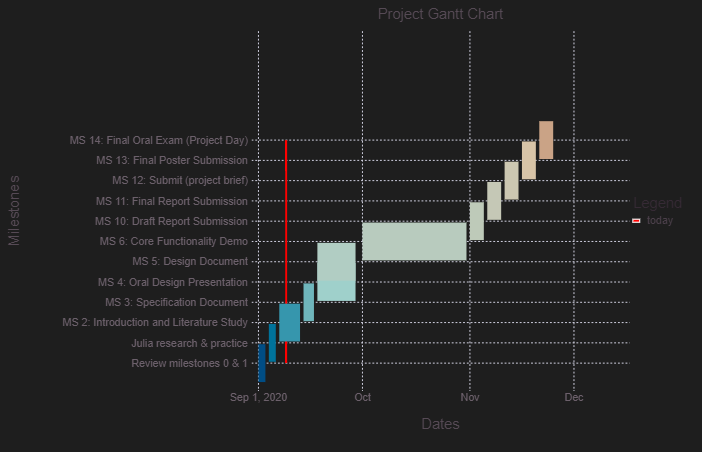
\includegraphics[padding=1ex,width=0.9\textwidth,frame]{img/gantt_chart.png}
    \caption{Project Gantt chart}
    \label{gantt_chart}
\end{figure}



\subsection{Preliminary Conceptual Design}\label{section_prelimConceptDesign}

Figure \ref{prelim_scd} shows the preliminary context diagram for the project.

\begin{figure}[h!]
    \centering % centers the figure
    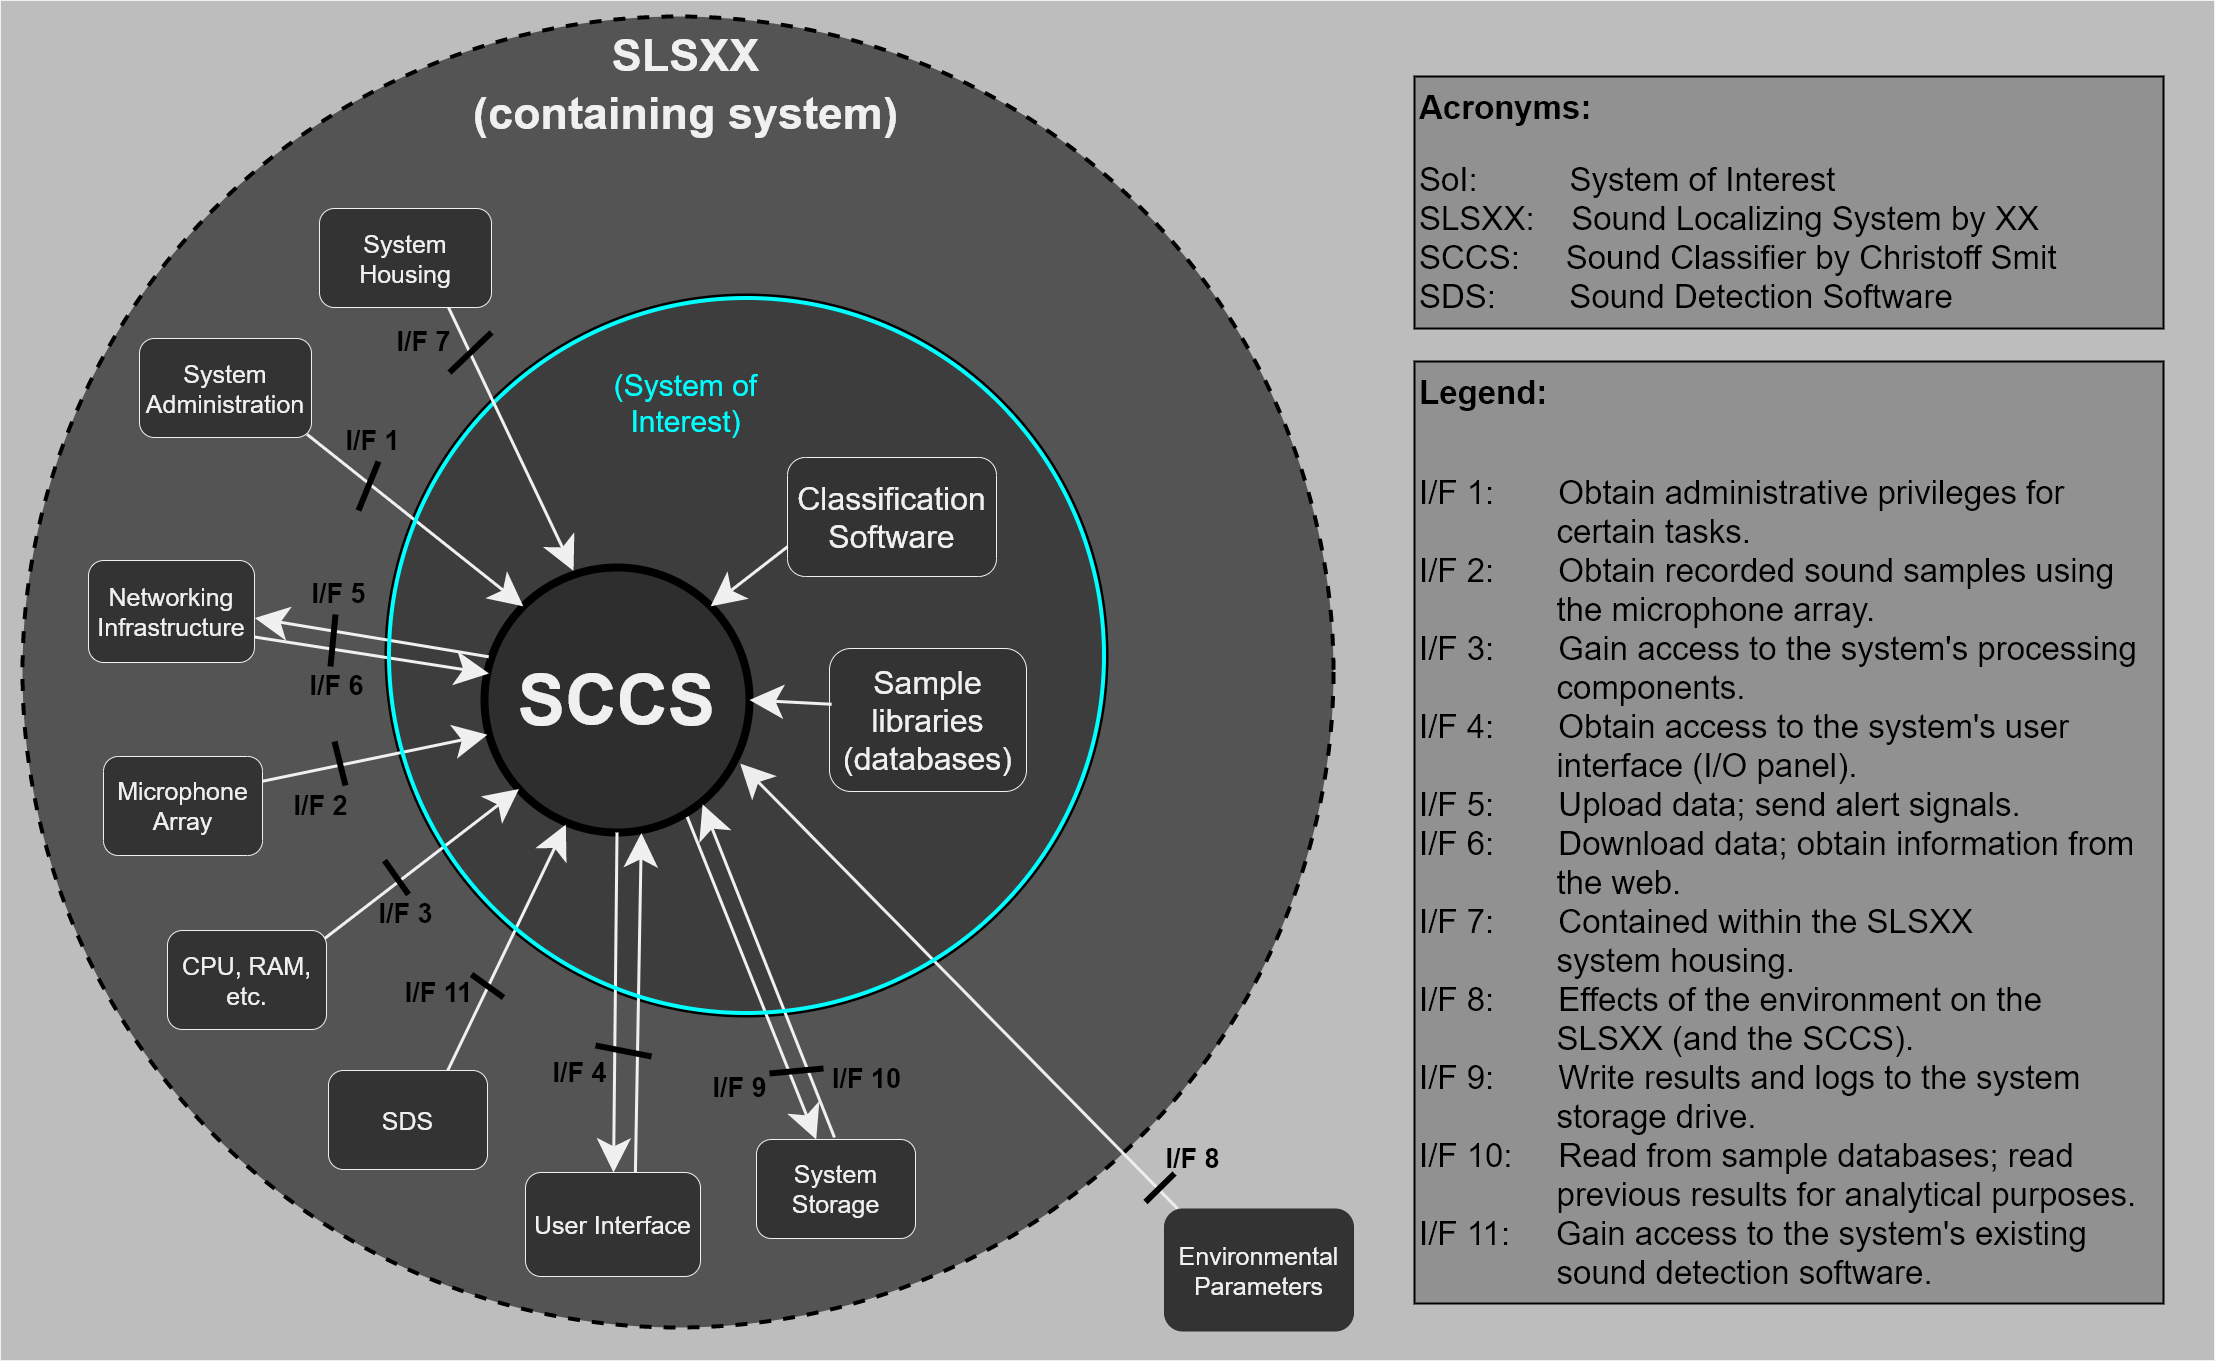
\includegraphics[padding=1ex,width=0.9\textwidth,frame]{img/prelim_scd.png}
    \caption{System Context Diagram (preliminary)}
    \label{prelim_scd}
\end{figure}


Figure \ref{prelim_physArch} shows the preliminary physical architecture of the system.

\begin{figure}[h!]
    \centering % centers the figure
    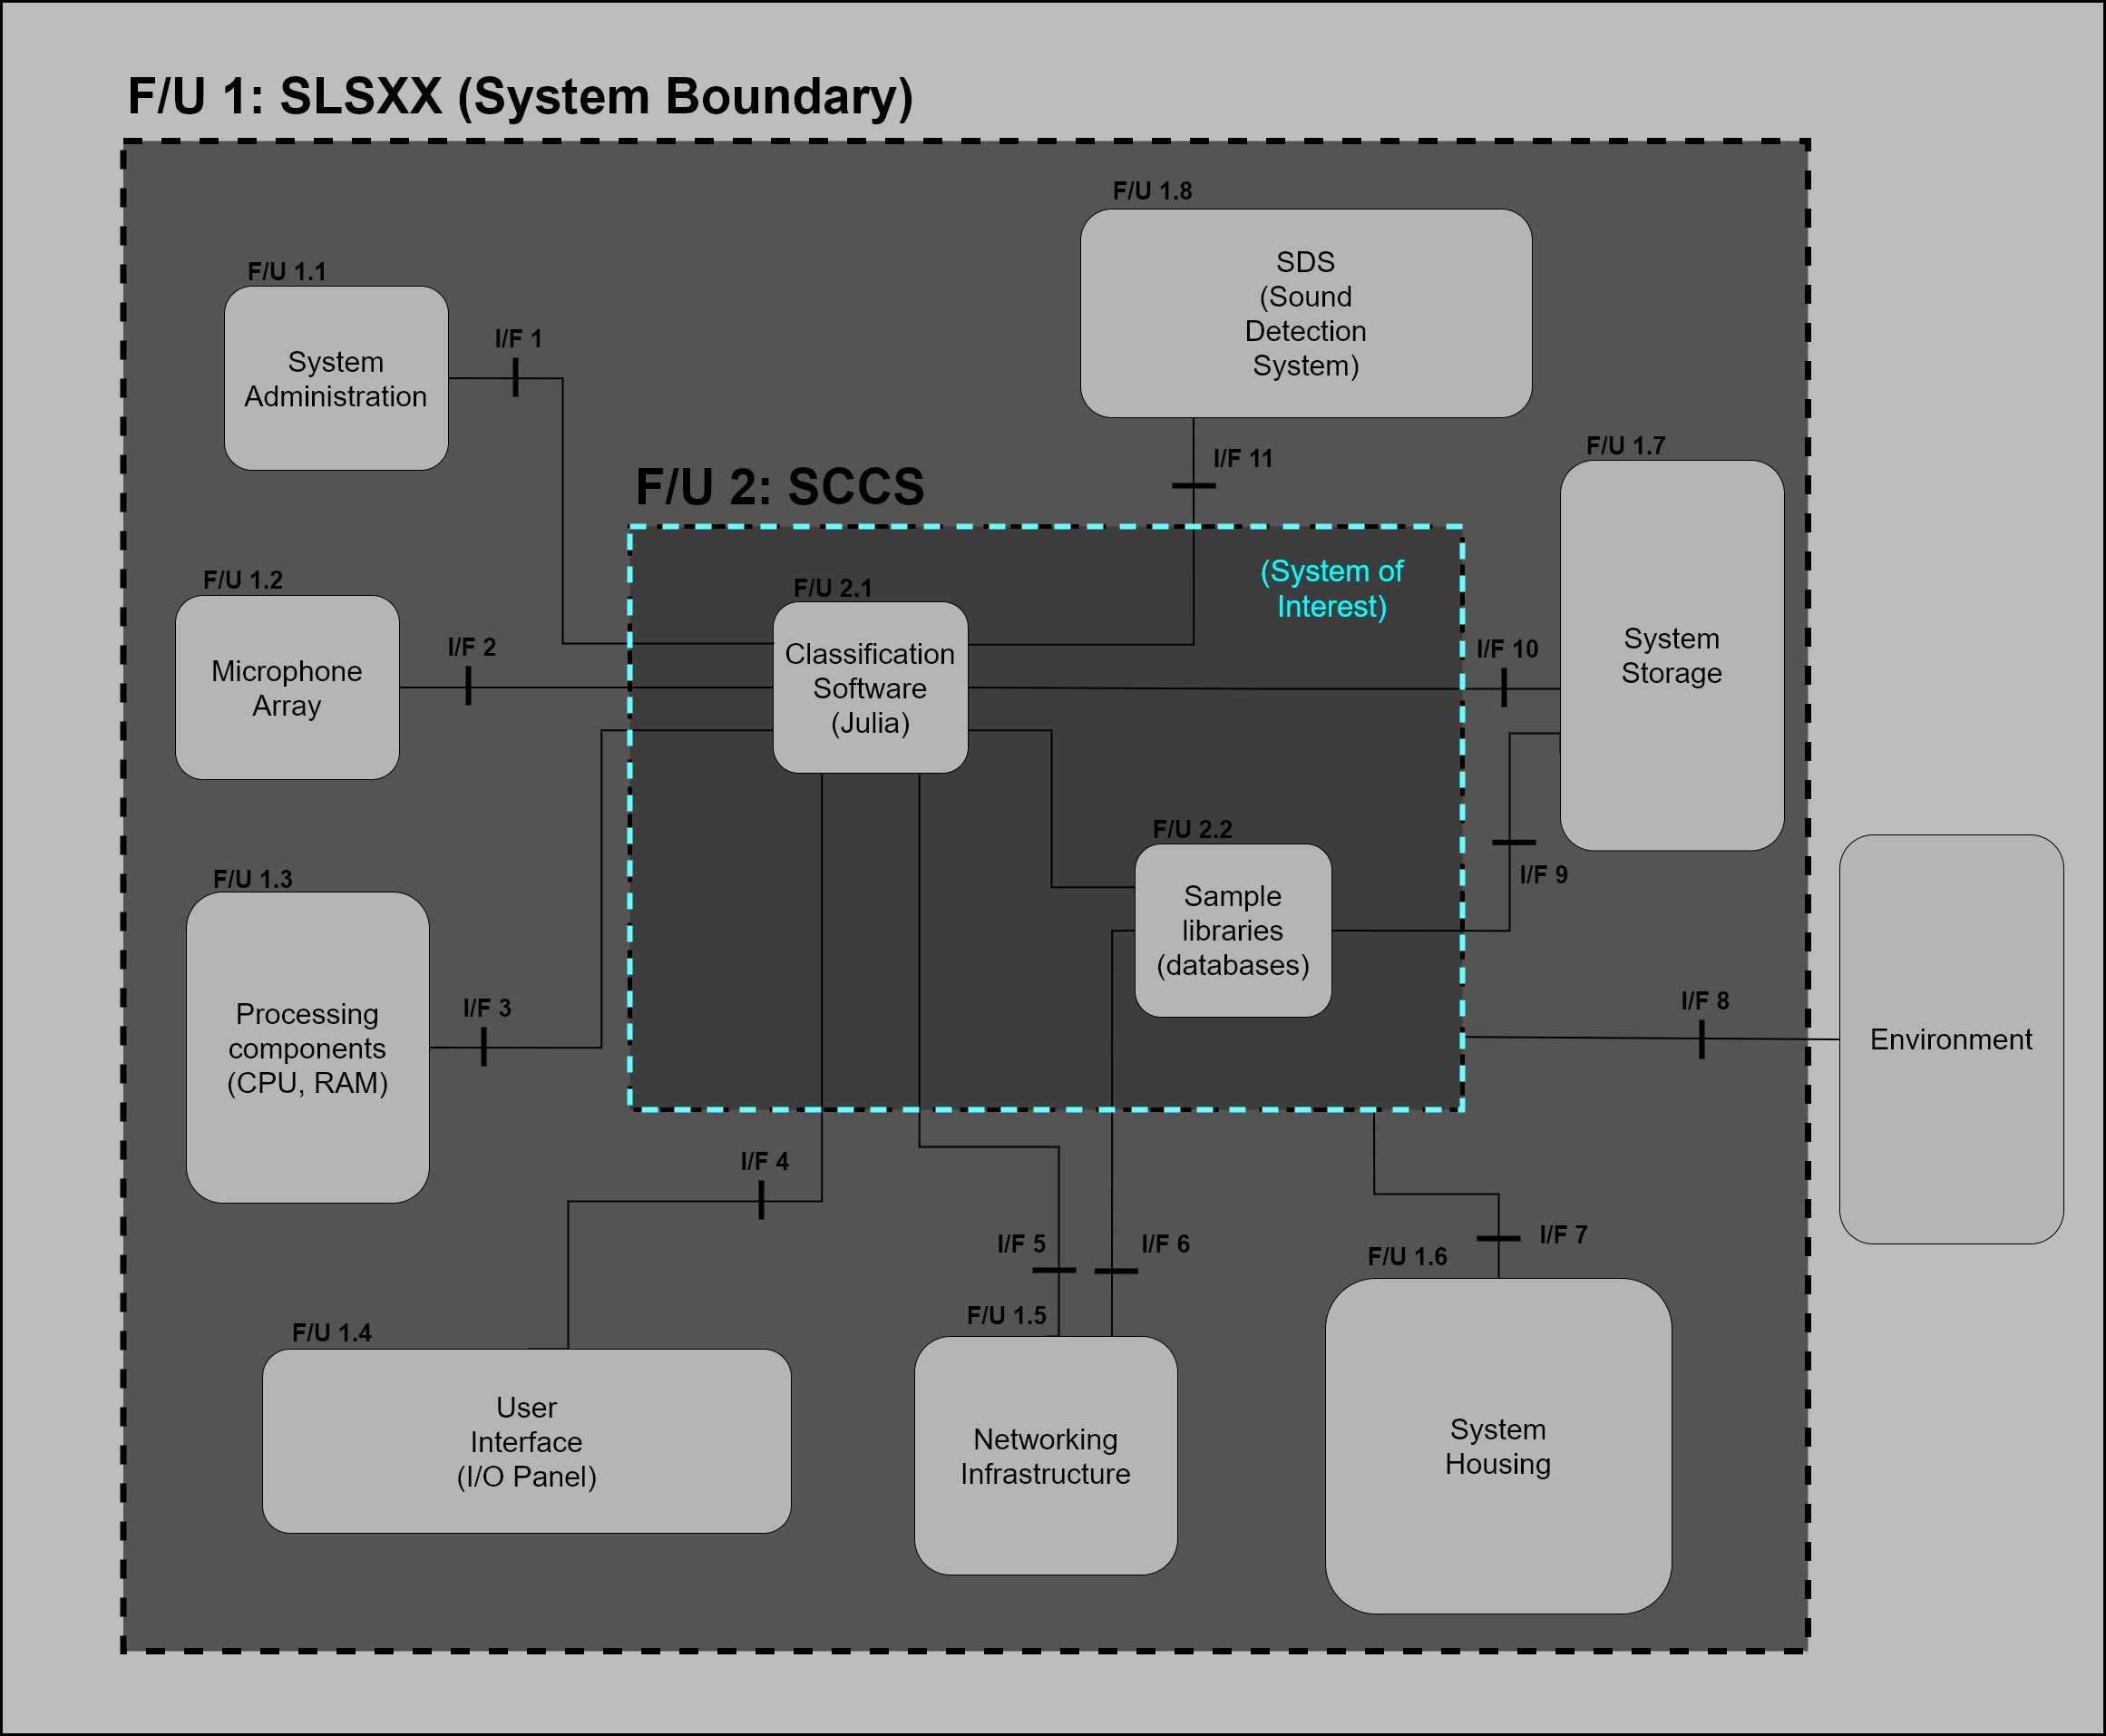
\includegraphics[padding=1ex,width=0.9\textwidth,frame]{img/prelim_physArch.png}
    \caption{System Physical Architecture (preliminary)}
    \label{prelim_physArch}
\end{figure}



Figure \ref{prelim_functFlow_full_life_cycle} shows the complete life cycle of the system.

\begin{figure}[h!]
    \centering % centers the figure
    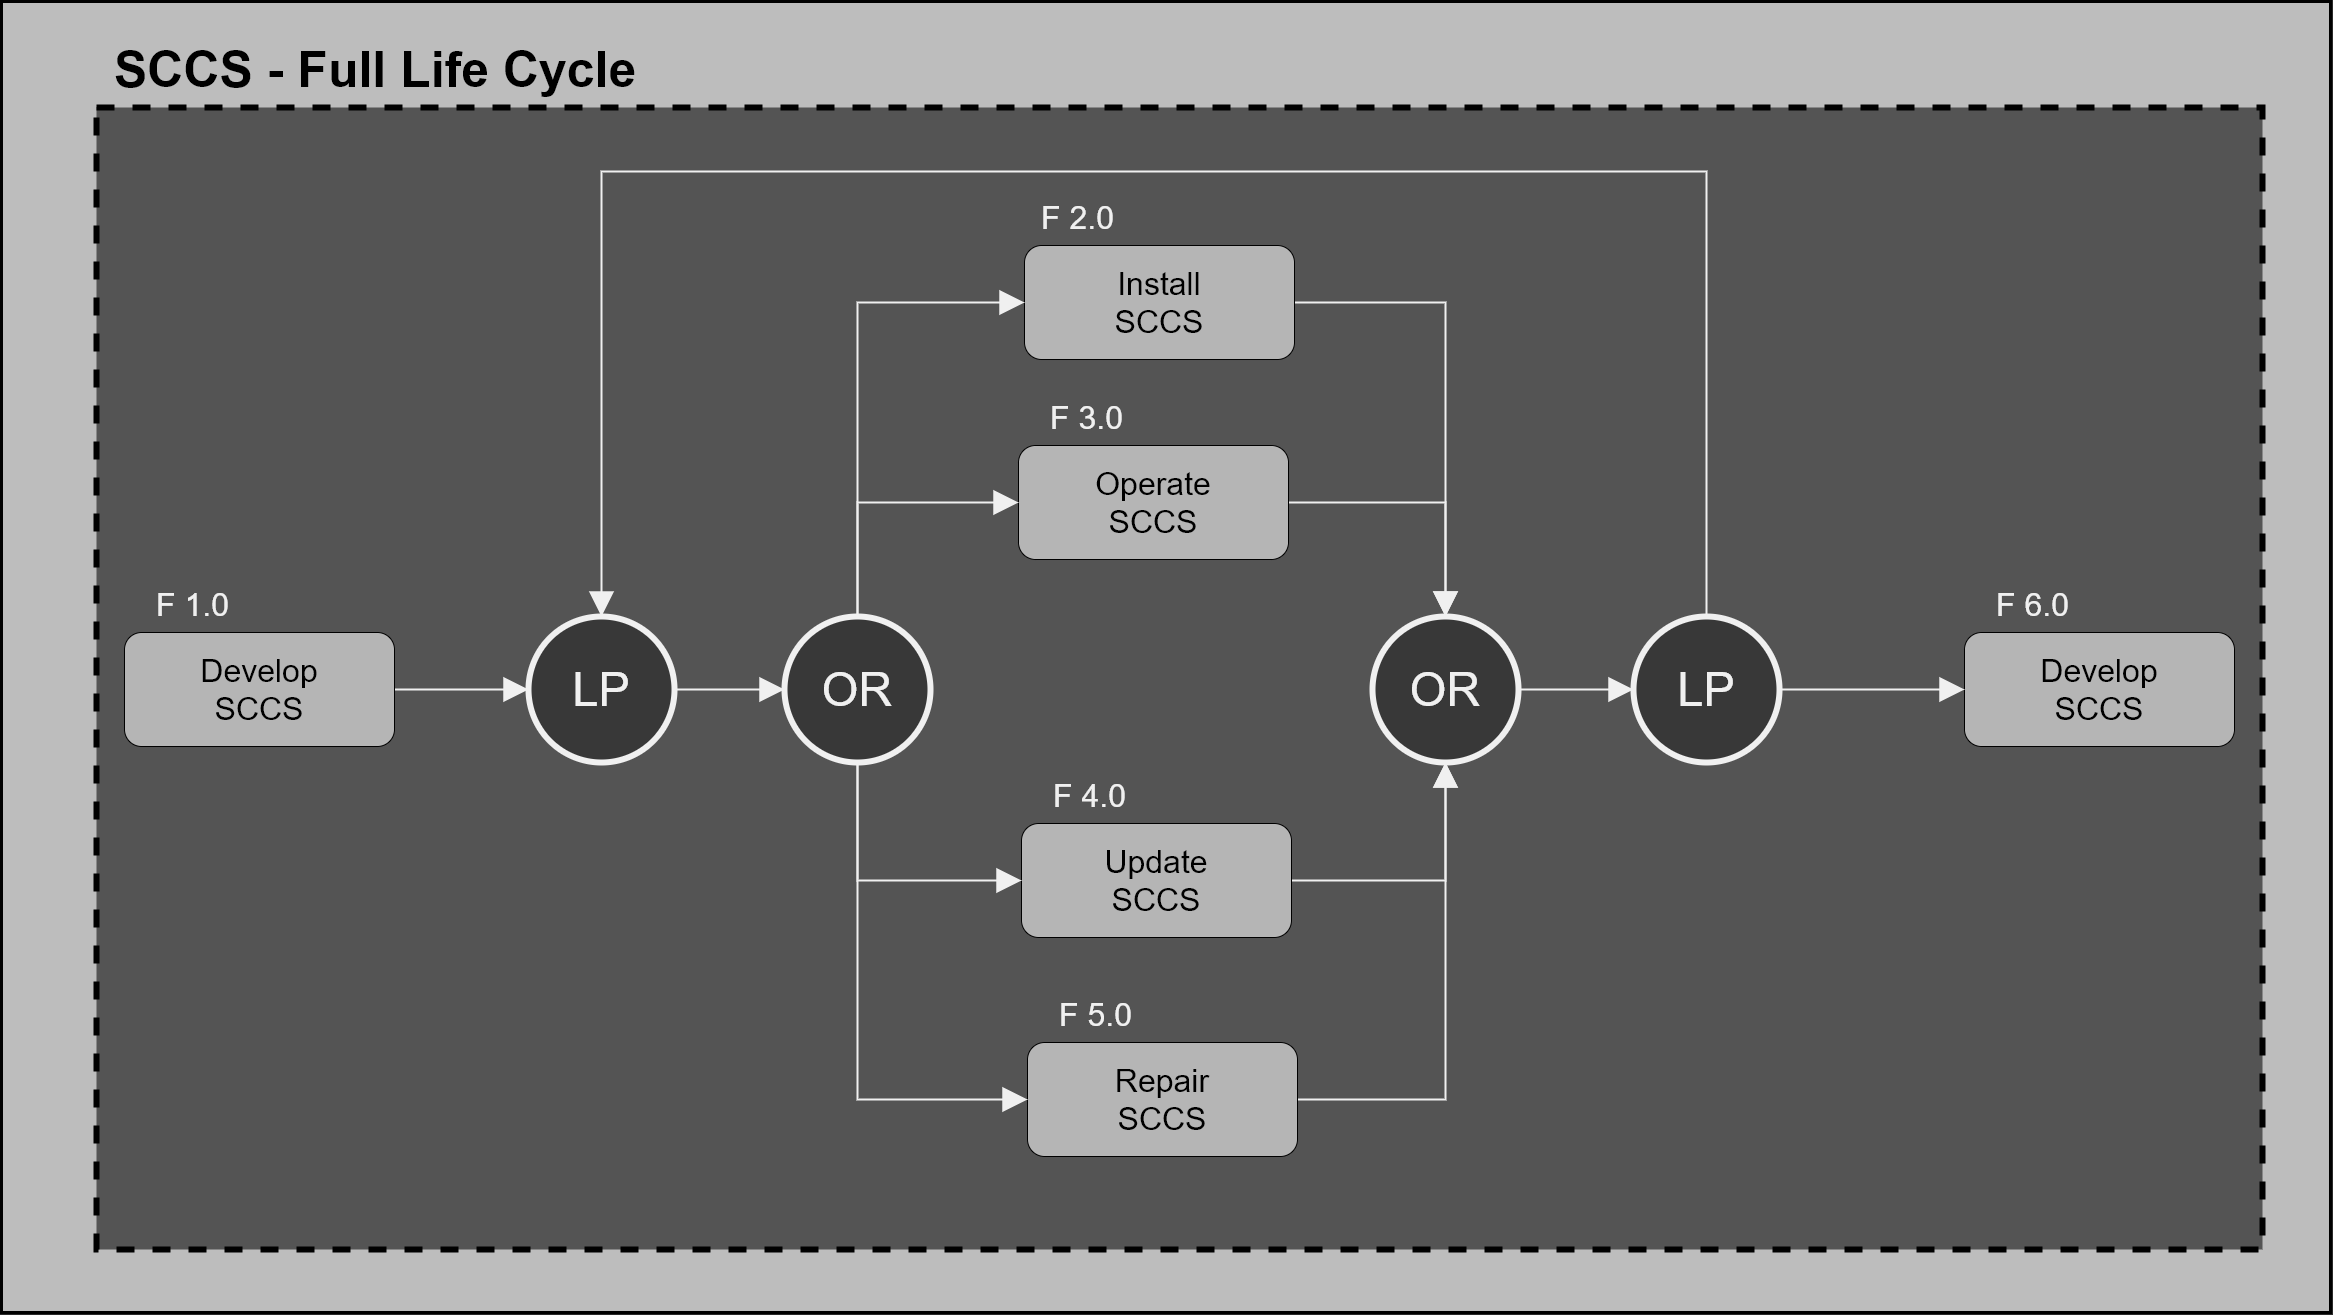
\includegraphics[padding=1ex,width=0.9\textwidth,frame]{img/prelim_functFlow_full_life_cycle.png}
    \caption{Full System Life-Cycle}
    \label{prelim_functFlow_full_life_cycle}
\end{figure}



Figure \ref{prelim_functFlow_F3_operate} illustrates the \textit{Operate} function in Figure \ref{prelim_functFlow_full_life_cycle}

\begin{figure}[h!]
    \centering % centers the figure
    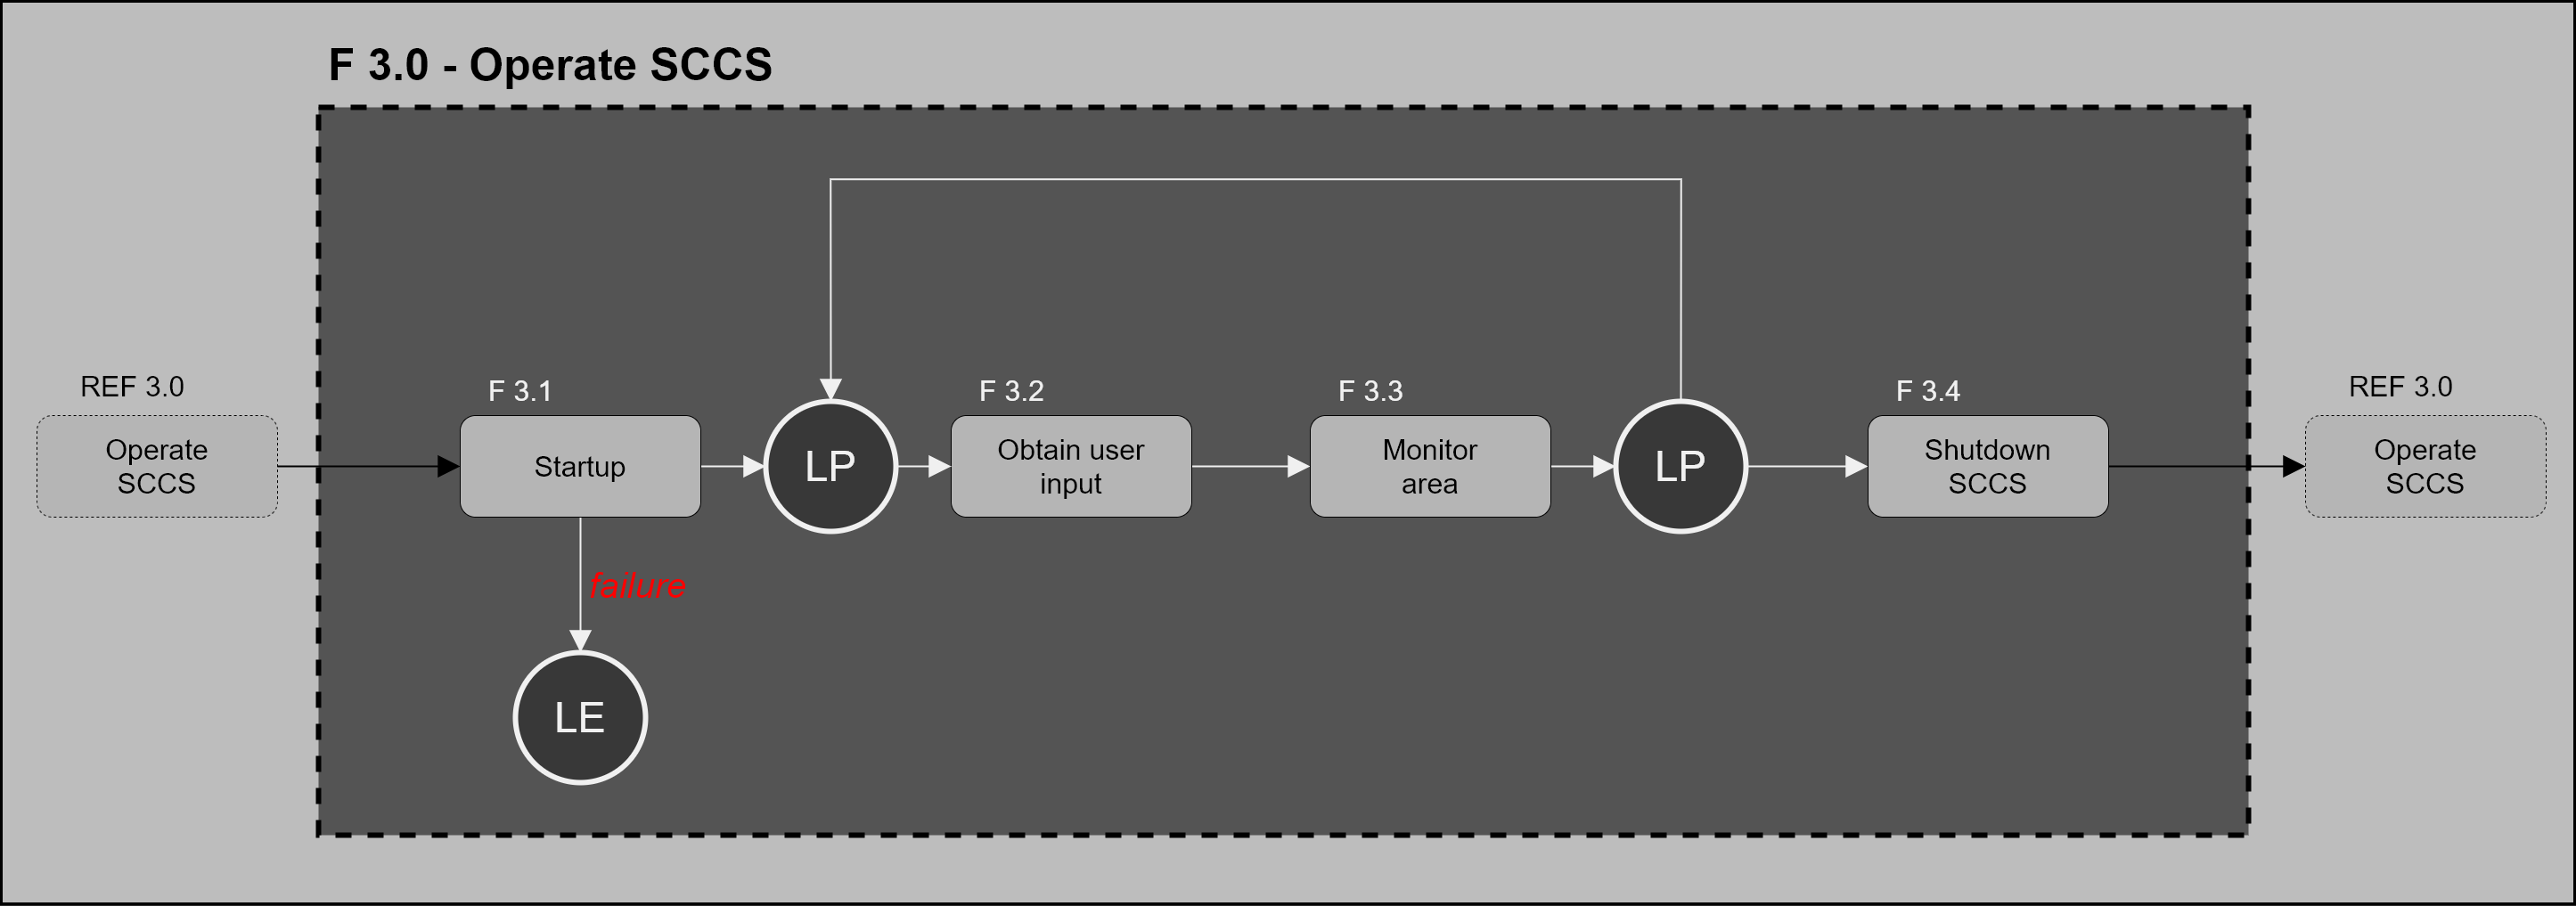
\includegraphics[padding=1ex,width=1.0\textwidth,frame]{img/prelim_functFlow_F3_operate.png}
    \caption{Function 3.0 - Operate SCCS}
    \label{prelim_functFlow_F3_operate}
\end{figure}



























%%%%%%%%%%%%%%%%%%%%%%%%%%%%%%%%%%%%%%%%%%%%%%%%%%%%%%%%%%%%%%%%%%%%
\newpage
\section{Literature Study}

This chapter entails an in-depth literature study of the project scope. A large part of the chapter is devoted to a technology survey which provides background on the functional units (main project components) identified in Figure \ref{prelim_physArch}.

\subsection{Introduction}

The detection and interpretation of sounds have been a part of humans' daily lives for thousands of years. Automatic detection and analysis of certain sounds may therefore be an appealing ability to introduce to a machine.

% Talk about the human ear and how it hears/detects sound


% The act of Audio surveillance\slash monitoring and why it is useful in security systems.

% How machine learning works and why it's being used for this project.

% The act of sound detection.

Sound may be recorded in a given number of channels, using a microphone with a specified bit-depth. The bit-depth indicates the amount of frequencies which may be uniquely identified by the sensor (microphone).

%TODO talk about sound (nearly) always coming in as a mixture of different sounds (possibly from different sources).

%TODO talk about sound being waves of air pressure, of which the vibrations are detected by a sensor (microphone) and converted to electrical voltage for performing the analog to digital conversion (ADC) process. In the end a discrete-sampled (digital) waveform is obtained. (mention Nyquist frequency here)



\subsection{General process (for audio machine learning)}
Figure \ref{wav_example} shows the WAV file recording of a dog barking 5 times over a period of 4 seconds.

\begin{figure}[h!]
    \centering % centers the figure
    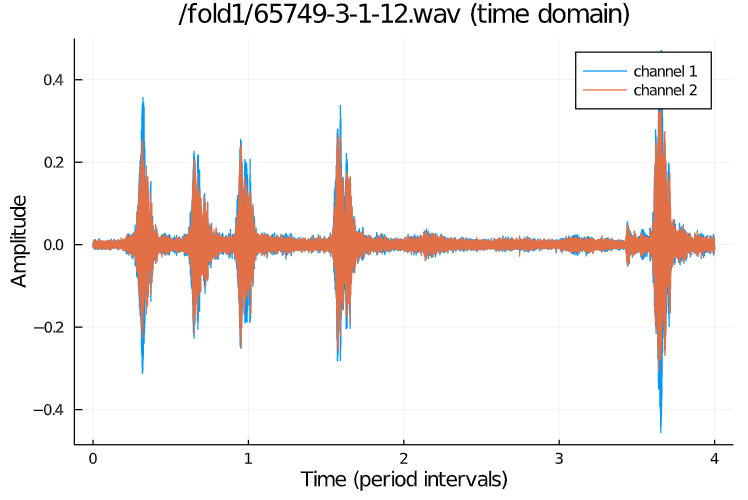
\includegraphics[padding=1ex,width=0.8\textwidth,frame]{img/wav_example.png}
    \caption{2-channel audio recording of a dog barking}
    \label{wav_example}
\end{figure}

%TODO the digital waveform is quantized in: time (44 100 Hz sampling rate of mic) and in amplitude (16 bit d.w.s 2^16 uniquely identifiable frequencies)

%TODO mention how it's safest (by avoiding artifacts and so on) to use an uncompressed format (i.e. WAV (and not MP3?)) for the audio samples.

%TODO mention that the 4s samples will be divided into a few different windows/segments (e.g. four 1s windows) -> to reduce the complexity of the machine learning algorithm. OVERLAP may be introduced with this windows (e.g. 50% overlap means the neural network will be considering most of the audio sample twice)

\newpage

The (Fast) Fourier transform is determined for the entire sample, providing an instantaneous ("snap-shot") illustration of the recording's total frequency content:

\begin{figure}[h!]
    \centering % centers the figure
    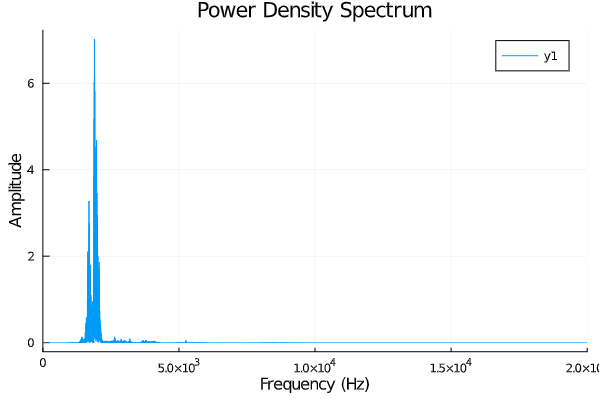
\includegraphics[padding=1ex,width=0.8\textwidth,frame]{img/fft_example.png}
    \caption{Periodogram (FFT) of the audio recording}
    \label{fft_example}
\end{figure}

It becomes apparent that the dog is mainly barking at a specific frequency around $2$ kHz.

Note that only frequencies up to $20$ kHz are considered. This is chosen in accordance with the average human hearing range, but also with the Nyquist frequency of the microphone in mind. The microphones used maintain a sampling frequency of $44.1$ kHz. Therefore, according to Nyquist's theorem, the highest frequency that each (of the three) microphones may accurately sample is $44.1/2=22.05$ kHz. %TODO consider downsampling as a pre-processing step

However, calculating the Fourier transform of the entire sound sample neglects the element of time, which is a very important characteristic in audio recording.

Consequently, the STFT (short-time Fourier transform) is calculated by determining the above-mentioned FFT at a few successive instances in time to produce the spectrogram in Figure \ref{stft_example}.

\begin{figure}[h!]
    \centering % centers the figure
    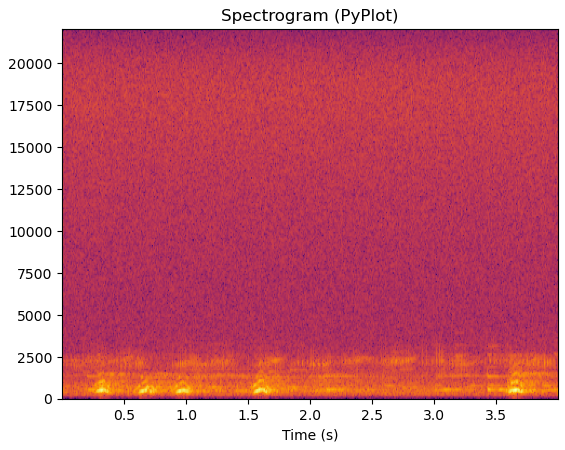
\includegraphics[padding=1ex,width=0.8\textwidth,frame]{img/stft_example.png}
    \caption{STFT (NFFT=512, noverlap=128)}
    \label{stft_example}
\end{figure}

Finally, the (logarithmic) Mel filterbank is applied to the signal, producing the two-dimensional array of MFCC's in Figure \ref{mfcc_example} that serves as input to the neural network. Note that $13$ coefficients are considered here with time windows of $25$ ms and a step size of $10$ ms. %TODO relate these window- and step sizes to the amount of samples per window/step (sodra uitgevind het wat die mics se specs is)

\begin{figure}[h!]
    \centering % centers the figure
    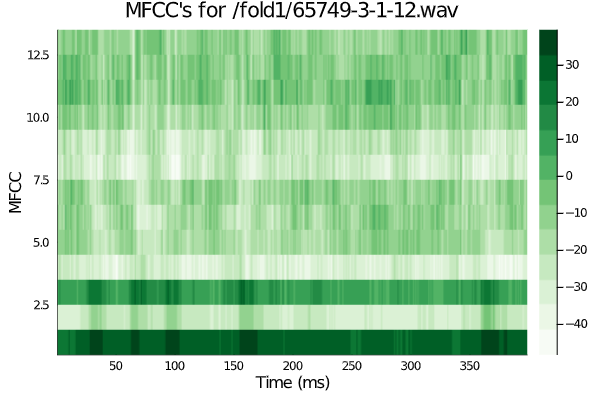
\includegraphics[padding=1ex,width=0.8\textwidth,frame]{img/mfcc_example.png}
    \caption{MFCC'c heatmap (N=13)}
    \label{mfcc_example}
\end{figure}

\subsection{Background}
%TODO discuss MFCC's a bit more
% 13 triangular filters with logarithmically ascending size (corresponding to the fact that human ears also prioritize lower frequencies)

%TODO mention AutoEncoders

%TODO mention Audio Embeddings (inspired by text embeddings), (uses a CNN "under the hood?") RECOMMENDED TO START HERE

%TODO praat oor (EN APPLY) Data Augmentation:
%Overlap tussen die 1s windows wat gesny word vanuit die 4 sec samples
%Time shift (and maybe stretch?)
%Frequency shift (and why stretching wouldn't make too much sense here, although a small amount e.g. 5% might be useful)
%adding Noise

%TODO mention AND APPLY dropout (first implemented by AlexNet in 2012)

%TODO mention AND APPLY early stopping

%TODO praat oor Normalization (LW nie hier relevant to softmax nie dit beteken iets anders e.g. om 'n wav file te normalize i.t.v. volume)

%TODO verduidelik softmax en hoe dit gesien kan word as die final activation function vir die neural net

%TODO praat oor CNN's en hoe hulle gebruik word vir CV

%TODO vind uit waarvoor staan MIR

%TODO praat oor Transfer learning (chopping off/using a pre-trained network (designed for some other use-case) and applying it to our problem). Mention hier hoe ons images se goed amper netso kan toepas op klank.
%LW dat die twee asse van 'n spectrogram verskil van 'n gewone image in die sin dat DIE TWEE ASSE VERSKILLENDE GOED verteenwoordig.
%Noem ook "images tend to be equivariant with respect to translation" en dat dit "weight sharing" allow

%TODO consider Long-Short Term Memory (LSTM) vs Transformers en hkm die latter beter is


\newpage
\subsection{Technology Survey}
%WaveNet (google speech assistant uses this)
%DeepConvNet (meant for images (Computer Vision (CV) models), but may be repurposed for sound)


\subsubsection{Trade-Off Studies}

% Do a technology survey on all the functional units (main components) in Figure prelim_phys_arch.

% Julia and why it offers a good environment for implementing machine learning.

% Flux and why it's chosen over TensorFlow/Keras
% (e.g. Flux only around 1000 lines of code, TensorFlow is over a million lines of code.... Flux written entirely in Julia, TensorFlow not).

% The specific microphones being used in the array and the influence of microphone quality. Mention the cost vs performance relationship.

%TODO include CNN's vs RNN's vs etc... (vergelyk verskillende tipe models; BEGIN BY 'N GEWONE PERCEPTRON)

%TODO include verskillende tipes optimizers

%TODO include verskillende activation functions (sigmoid vs relu)










% FROM HERE ON, NO PROJECT MANAGEMENT CONTENT IN THE REPORT...
%%%%%%%%%%%%%%%%%%%%%%%%%%%%%%%%%%%%%%%%%%%%%%%%%%%%%%%%%%%%%%%%%%%%
\newpage
\section{System Design}
% What should be done to solve the problem (i.e. THE PLAN)?





%%%%%%%%%%%%%%%%%%%%%%%%%%%%%%%%%%%%%%%%%%%%%%%%%%%%%%%%%%%%%%%%%%%%
\newpage
\section{Detail Design and Implementation}
% What should be done to solve the problem (i.e. THE PLAN)?






%%%%%%%%%%%%%%%%%%%%%%%%%%%%%%%%%%%%%%%%%%%%%%%%%%%%%%%%%%%%%%%%%%%%
\newpage
\section{Testing and Evaluation}
% Testing and evaluation of your plan
%TODO show graph of accuracy for classifier on test data
%TODO wys hoe 'n sample self opgeneem (en gelabel) is in Audacity e.g. 'n hond :D







%%%%%%%%%%%%%%%%%%%%%%%%%%%%%%%%%%%%%%%%%%%%%%%%%%%%%%%%%%%%%%%%%%%%
\newpage
\section{Conclusion \& Recommendations}


\textit{Christoff Smit - \today}




%%%%%%%%%%%%%%%%%%%%%%%%%%%%%%%%%%%%%%%%%%%%%%%%%%%%%%%%%%%%%%%%%%%%
% REFERENCES:
\clearpage
\newpage
\addcontentsline{toc}{section}{References}
\printbibliography
%TODO kyk na references by 33:43 van https://www.youtube.com/watch?v=uCGROOUO_wY&t=672s



%%%%%%%%%%%%%%%%%%%%%%%%%%%%%%%%%%%%%%%%%%%%%%%%%%%%%%%%%%%%%%%%%%%%
% APPENDICES:
\clearpage
\newpage
\section*{Appendices}
% \addcontentsline{toc}{section}{Appendix A: Matlab code}
% \lstinputlisting[style=Matlab-editor]{submission.m}

\end{document}